\section{The Peer-to-Peer Network Architecture}
In the peer-to-peer network architecture, every node in the network
contributes with its resources, including both storage space and
processing power.

Popularised through file sharing, found its way into academia, dhts,
distributed systems

\section{Gossiping}

\section{The Publish-Subscribe Communication Paradigm}

Publish-Subscribe is a fully asynchronous, loosely coupled,
highly scalable, event-based messaging pattern. There are three main
system components in the pub/sub interaction scheme: the publishers, the
subscribers and the event service. The publishers publish events, and
the subscribers subscribe for events, while the event service handles
managing both subscriptions and publications, as well as routing events
to the subscribers. The basic architecture of a typical pub/sub system
is outlined in Figure~\ref{fig:pubsubarch}.

\begin{figure}
\centering
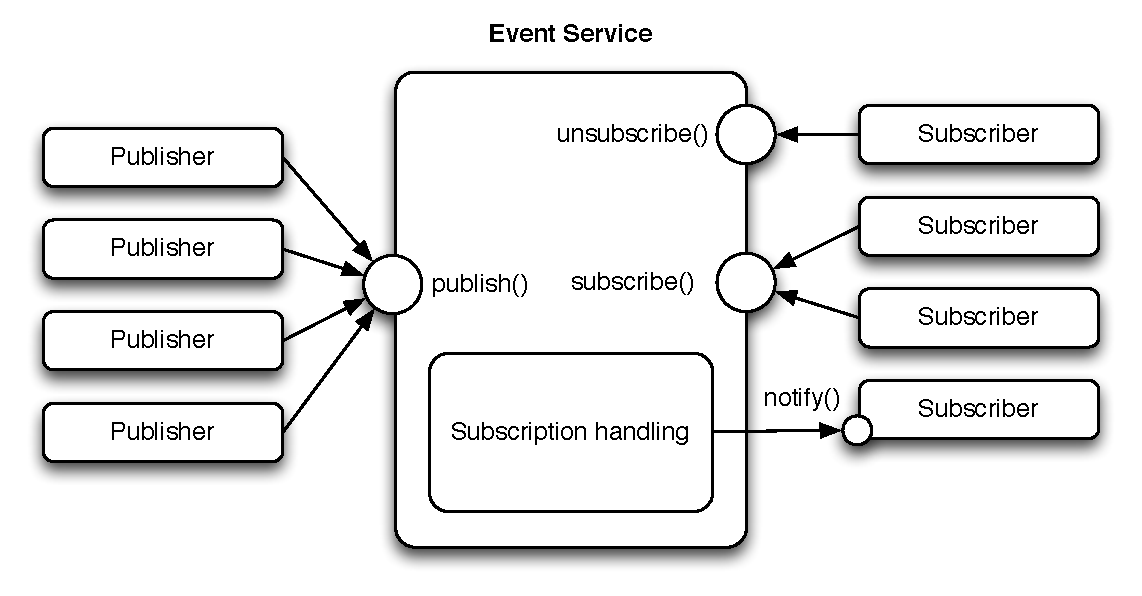
\includegraphics[width=\textwidth]{figures/pubsubarch}
\caption{The basic architecture of a pub/sub system.}
\label{fig:pubsubarch}
\end{figure}

The event service functions as an intermediary between publishers and
subscribers. It provides a level of indirection, as well as an service
interface. Publishers are able to generate new events through the
\texttt{publish} service call. It is now the responsibility of the event
service to determine which subscribers are interested in receiving this
event, and how to route the event to them. The subscribers register
their interest through a \texttt{subscribe} service call. The event
service will then store each subscribers interest in order to
disseminate events correctly. The publishers are then able to cancel
their subscriptions through a \texttt{unsubscribe} service call. No
information is forwarded from subscribers to publishers or from
publishers to subscribers.

The pub/sub paradigm provides a higher degree of decoupling than other
traditional approaches. In general there are three types of decoupling
pub/sub system provides us with:

\begin{description}
  \item[Space decoupling] The publishers and subscribers does not need to
    know about each other.
  \item[Time decoupling] Events are delivered regardless of whether or
    not publishers and subscribers are online at the same time.
  \item[Synchronization decoupling] Neither publishers nor subscribers
    are blocked when attempting to perform their operations.
\end{description}

While many other approaches can provide the first two forms of
decoupling, the main advantage of pub/sub is its fully asynchronous nature.
Approaches such as tuple spaces or message queues cannot completely
provide this synchronous decoupling, as messages are retrieved in a
synchronous manner. This property is key to the suitability for pub/sub
in large distributed system.~\cite{Eugster:2003}

\subsection{Message Filtering in Pub/Sub}

The subscription semantics of the pub/sub paradigm plays an important
role in the performance and flexibility of the system as event messages
are routed and managed based on topic or content. There are three
distinct types of subscription schemes:

\begin{description}
  \item[Topic-based] Events are split into topics, usually represented by
      a string.
  \item[Type-based] Filters events based on the structure of the data.
      Provides type safety at compile time.
  \item[Content-based] Events are filtered based on a global
      list of universal event attributes.
\end{description}

Content-based provides better expressiveness in terms of filtering out
the relevant events. However, this comes at the cost of higher overhead
with regards to handling subscriptions. The complex filtering algorithms
limit the scalability of such systems with regards to the number of
subscriptions. Type based is similar to content-based in the sense that
the public members of the types together form a description of the
content of the event. Although this ties the implementation of the
pub/sub system closer to the programming language, it still suffers from
the same drawbacks as content-based.

Topic-based offer less expressiveness than the other two subscription
schemes, but better performance if the set of possible event properties
is limited. Also, topic-based is more suited for dissemination and
multicasting, as topics can be thought of as groups, where subscribing
to topic T can be equivalent to joining the group for that topic. This
is a common approach taken by several proposed pub/sub
systems\cite{needs citation}.

Traditionally, reliable multicasting of data through deterministic
dissemination has been the common approach. However, more recent
implementations investigate the potentials of probabilistic protocols,
which are more suited to the nature of decentralized systems and P2P.
These protocols do not guarantee full reliability, but provides a high
quantifiable \emph{probability} that events are delivered to all
subscribers.

\section{Online Social Networks}
What is an OSN?\ Impact on networks?\ What approaches?\ Decentralised OSNs?

\section{Social Network Analysis}
What is SNA?\ What are the common characteristics of a Social Graph?\
Actors, How to measure influence/power of actors (centrality?)

\section{Pub/Sub in Online Social Networks}

\section{The Gephi Open Graph Viz Platform} Gephi~\cite{ICWSM09154} is
an open source tool for exploring and visualizing all kinds of networks,
including dynamic and hierarchical graphs. Described by the authors as
``photoshop for graphs'', Gephi enables the user to interact with the
graph structure, as well as manipulate the colors and sizes of the
visual graph representation in order to display graph properties in an
intuitive way. Gephi aims to help researchers and data analysts in
discovering patterns and revealing hidden properties of the graph in
question, as well as easily discovering errors in the dataset. Gephi
also provides a set of statistical tools for measuring common metrics
for Social Network Analysis~(SNA) such as centrality, as well as metrics
useful for general graph topology analysis such as degree, path length
and clustering coefficient. Gephi is also useful in the emerging field of
Dynamic Network Analysis~(DNA)  as it supports temporal graphs,
giving the user the ability to filter the graph model according to a
defined time interval. It also support playback of the graph evolution,
as well as visualizing changes to graph data over time through size,
color and text labels which can be applied to both nodes and edges.

Gephi provides a rich GUI-experience where users may interact with the
graph representation, apply layout algorithms, filter the graph
representation, execute metrics, apply color and size based on graph
properties and animate the graph evolving over time through the timeline
component.  The Gephi software architecture is highly modular and
supports extensions via plugins, some of which are available in a
official plugin marketplace found at~\cite{gephimarketplace}. New
metrics, filters or database support may be implemented through such
plugins by developers and published to the marketplace free of charge.

\begin{figure}
\centering
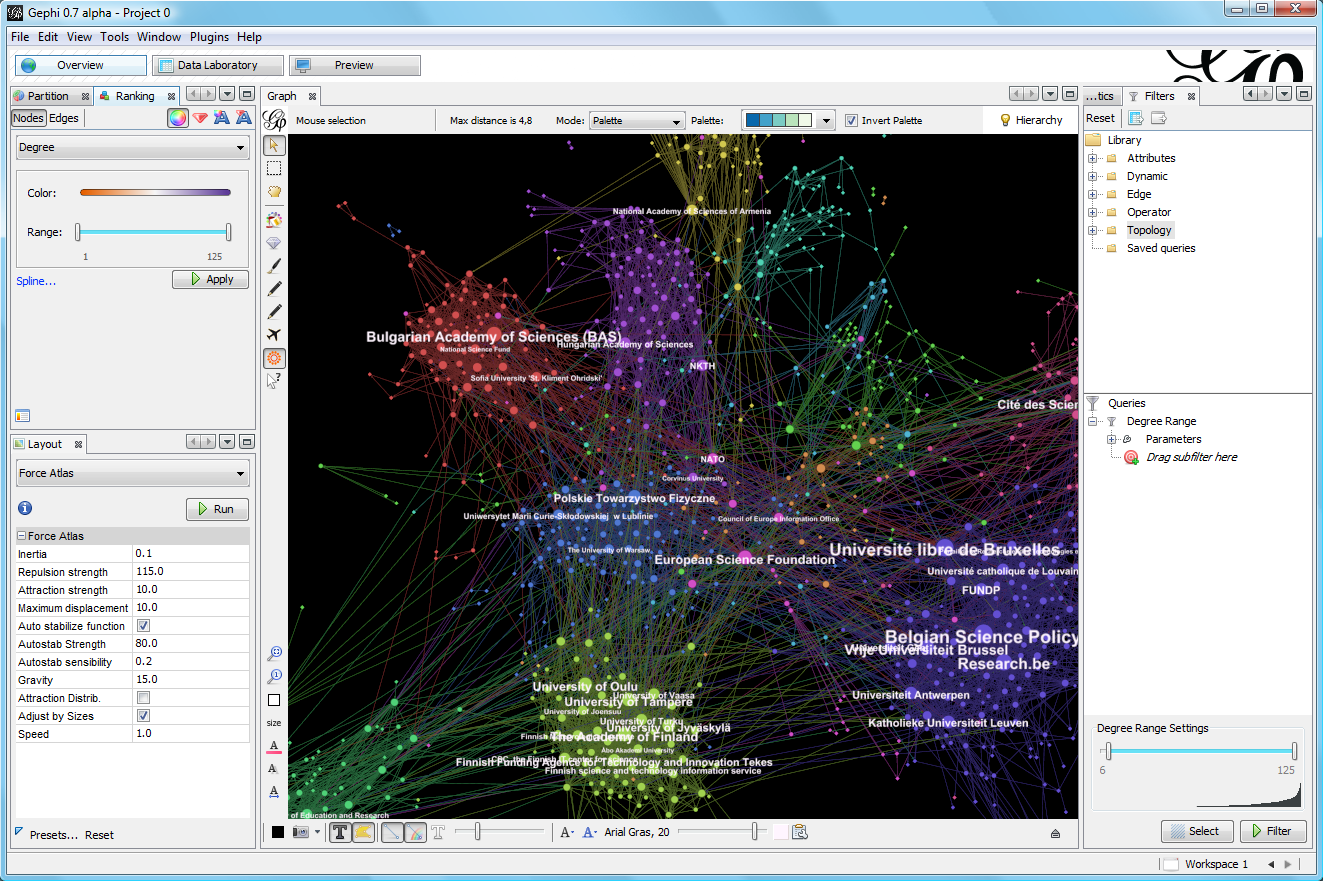
\includegraphics[width=\textwidth]{img/gephi1}
\caption{The Gephi Tool supports
visualization of graphs through coloring and sizing the visual graph
representation. It also enables adding labels to nodes and edges. In
this screenshot, Gephi is used to detect and visualize
communities.}
\label{img:gephi1}
\end{figure}

We consider tools such as Gephi to be a valuable addition to the field
of P2P protocol research. Visual Exploration of a dynamic network graph
is a useful approach to evaluating these protocols, as some properties
of the system are more easily spotted visually. For example, during our
implementation work, it was trivial to visually confirm that some edges
were missing from the graph, leading to the discovery of a critical bug
in the implementation code which would otherwise be difficult to spot.
It is also worth to note that the different actors involved in the Gephi
project has formed a legal entity in the form of The Gephi
Consortium~\cite{gephi-consortium} in order to assure future development
of this tool. This provides us with a certain degree of assurance that
this project is something well worth investing in, as the risk of it
being discontinued seems unlikely at this point in time.

\section{The Gephi Toolkit}

In addition to the GUI-client, the authors of Gephi also provide an API
through the Gephi Toolkit project. The toolkit packages essential
modules from the GUI-client into a standard Java library which can
be used by any stand-alone Java project by including it as a dependency.
We take advantage of this toolkit in our implementation work, where it
is mainly used to handle and store reports collected from PeerNet
simulations.

\section{The GEXF File format}

The GEXF (Graph Exchange XML Format) file format~\cite{gexf} is an
effort by the Gephi Consortium to define a standard language describing
complex network structures. Being developed by the same group of people,
the Gephi Tool is naturally fully compatible with this format, and is
able to both import and export GEXF files. This is also the case with
the Gephi Toolkit, as the module for handling such imports and exports
are included in this toolkit as well.

The GEXF file format is able to describe a graph through its nodes and
edges, as well as any data and dynamics associated with the graph. More
specifically, the file format is able to describe node, edges and their
associated attributes. Listing~\ref{lst:gexf-basic} provides an example
of a minimal static GEXF file, describing nodes, edges and attributes of
a graph.

\begin{figure}
\lstinputlisting[language=XML, label=lst:gexf-basic, frame=single]{listings/basic.gexf}
\caption{A GEXF description of a minimal static graph}
\end{figure}

\subsection{Dynamics}

One of the major advantages of this file format is its support for
dynamic functionalities.  Both nodes, edges and attributes may have a
defined time interval where they exist. These lifetime intervals are
described as ``spells'' if applied to nodes and edges, and as ``start''
and ``end'' XML-attributes if applied to node or edge attributes. The
GEXF file in Listing~\ref{lst:gexf-dynamics} shows an example of a
dynamic graph where spells are used in order to determine the lifetime
of the nodes.  The start and end times are by default encoded as
doubles, however, dates are also supported, as seen in this example.

The
support for dynamic graphs makes this file format an interesting option
for storing simulation data, and in our implementation work we use this
format extensively as part of our research effort.

\begin{figure}
\lstinputlisting[language=XML, caption={}, label=lst:gexf-dynamics,
frame=single] {listings/dynamics.gexf}
\caption{Example of  dynamic GEXF file using spells}
\end{figure}

\section{The PeerNet Simulator}

\subsection{Event Engine}

\subsection{Protocols}

\subsection{Observers}

